\chapter{软件需求规格说明书}
\section{引言}

\subsection{编写目的}

  
本文档的目的是详细地介绍饿了吧APP所包含的需求,以便客户能够知晓产品的确切需求以及开发人员能够根据需求进一步进行扩展开发,以下叙述将结合文字描述、数据流图、ER图等来描述饿了吧APP的功能、性能、用户界面、运行环境、外部接口以及针对用户操作给出的各种响应。本文档的预期读者有客户、开发人员等。

\subsection{背景}

  
该项目适用于喜欢吃餐厅菜肴但不喜欢出门或不善于做饭的各年龄段人群,由谢帛洋和杨宇鑫二人团队进行开发和部署。

\subsection{参考资料}

{[}1{]}窦万峰.软件工程方法与实践(第三版).北京:机械工业出版社,2016

{[}2{]}普莱斯曼.软件工程:实践者的研究方法(原书第8版).北京:机械工业出版社,2016

\section{任务概述}

\subsection{项目概述}


\subsubsection{项目简介}
  
饿了吧APP是一款针对各年龄段各类人群的外卖软件,大家可以在这里浏览各个餐厅的美食,以及足不出户享受菜肴。软件最大的特色是添加了AI智能咨询服务,输入需求就可以得到饮食建议,方便使用者进行选择。

\subsubsection{项目目标}

  
该项目的市场目标为以年轻人群体为主、外卖软件市场,应用目标为实现外卖以及饮食咨询工作。

\subsubsection{具体功能概述}


(1)搜索功能:通过餐厅名、餐品名或地址模糊搜索显示结果列表。

\begin{quote}
(2)点餐功能:进入餐厅后可以选择餐品加入购物车,点击购物车可以看到餐品明细,继而可以进行餐品支付。
\end{quote}

(3)咨询功能:可以询问智能AI得到推荐食谱。

(4)订单功能:可以显示未支付和已支付的所有订单,并能查看订单明细。

(5)我的信息:查看个人基本资料,可以进行个人资料的修改(包括电话、头像等)。

(6)商家功能:可以进行商家注册以及登录,登陆后可以上架商品,编辑商品信息等。

(7)点赞、收藏和评论功能:在商家列表页可以进行点赞、收藏以及评论功能。

\subsection{用户特点}

  本产品的用户主要是喜爱点外卖年轻人群体,接受新鲜事物的能力比较强,他们比较容易接受外卖菜肴。并且对于智能AI的认可度也比较高。尤其是当代有许多人比较`宅',这类人群是我们的重点目标客户。

\subsection{假定和约束}


(1)人力和时间的约束:本APP开发过程中需要考虑到人力和时间的约束,相较于一些软件的开发团队来说人员较少时间较短。

(2)技术发展的约束:计算机技术和发展的日新月异,将会给信息处理带来更多手段,同时也会带来更加丰富的信息表达形式,例如心形的人工智能等等,可能导致我们的搜索时候没有那么智能,这就要求软件在设计时要考虑技术变化的可能性,为可能的变化预留一定的处理能力。

\section{功能需求}

\subsection{功能划分}

1)饿了吧的顶层数据流图

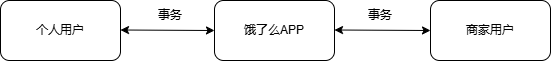
\includegraphics[width=5.73958in,height=0.63542in]{Picture30}

           图 1饿了么顶层数据流图

  
描述:如图1所示,用户可以扮演两种角色------个人用户、商家用户。当用户选择个人用户时,可以向饿了么发送事务(如修改资料等),同时个人用户可以浏览饿了么返回的事务,即个人用户与饿了么有双向的数据流动。当用户选择商家用户时,可以向饿了吧系统发送事务上架商品,同时可以浏览饿了吧返回的事务,即商家用户与饿了吧系统也有双向的数据流动。

(2)饿了吧的0层数据流图

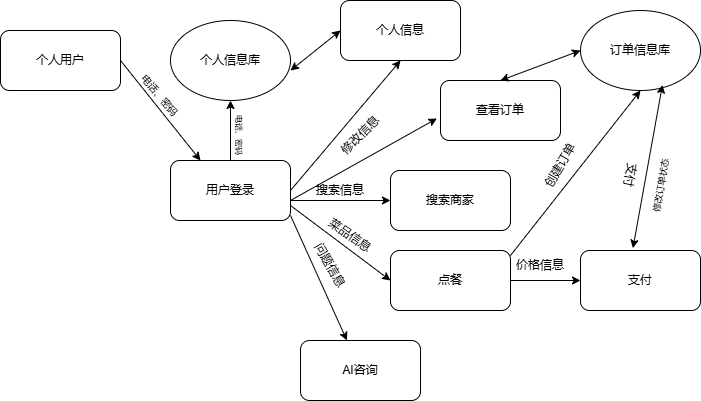
\includegraphics[width=5.76111in,height=3.29583in]{Picture31}

           图 2 饿了吧 0层数据流图

  
描述:如图2所示,个人用户通过提交身份信息向用户登录事务发送请求。用户登录事务从用户信息库中读取相应的用户信息进行匹配判断登录结果。用户登录成功后,用户可以进行个人信息管理、搜索商家、点餐、AI咨询、查看订单等操作。用户进行搜索操作时,用户提供的搜索信息流动到搜索事务,搜索事务对搜索信息进行相应的处理后得到商家信息。用户进行个人信息管理时,用户的修改信息传入信息修改事务中,修改个人信息库并返回修改后的新信息。进行点餐操作时发送菜品信息并进入支付事务,支付事务修改数据库创建新订单。其他操作同上述基本一致。

\subsection{功能描述}

(1)用户登录

​
功能描述:如图3所示,用户登录可以分为注册和登陆。注册时用户提供新用户注册信息发往注册事务,注册事务根据新用户注册信息得到新用户信息存入用户信息库,同时流动出用户信息。登录时用户提供用户名和密码发往登录事务,登录事务将得到的用户名和密码与用户信息库中的信息匹配,同时流动出用户信息。

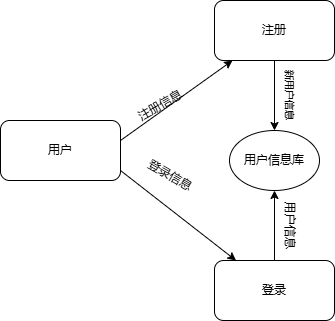
\includegraphics[width=2.94236in,height=2.81944in]{Picture32}

  图 3 用户登录功能细化数据流图

(2)个人信息管理

​
  功能描述:用户登录后可以进行相应操作进入个人信息管理界面,用户可以在此页面修改自己的个人信息。

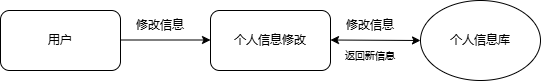
\includegraphics[width=5.63542in,height=0.84375in]{Picture33}

            图 4 个人信息管理功能细化数据流图

(3)搜索商家

​
功能描述:如图4所示,用户在搜索栏输入相应的搜索信息。搜索信息可以是商家名称或菜品名称。用户进入搜索商家事务,搜索商家事务处理传入的搜索信息流动出商家内容。

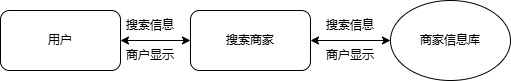
\includegraphics[width=5.32292in,height=0.84375in]{Picture34png}

           图 5 搜索功能细化数据流图

(4)点餐功能

​  
功能描述:用户选择菜品后提交菜品信息触发点餐事务,创建订单修改订单信息库,接着触发支付事务改变订单状态值。

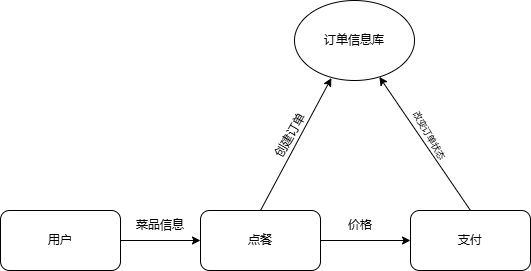
\includegraphics[width=4.22222in,height=2.15486in]{Picture35}

图 6 点餐功能细化数据流图

(5)咨询功能

​  功能描述:用户可以向智能AI传递问题信息,触发咨询事务,返回AI的回答。

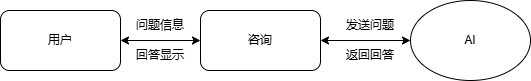
\includegraphics[width=5.53125in,height=0.84375in]{Picture36}

             图 7 咨询功能细化数据流图

(6)订单功能

  功能描述:用户点击订单后触发订单查看事务,事务从订单数据库查找订单数据并分为已支付和未支付,进行显示。

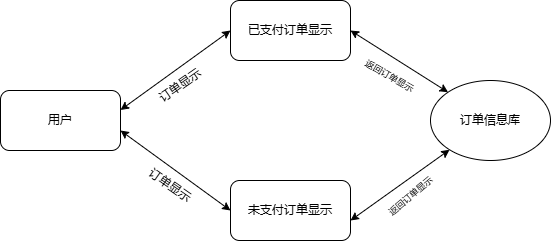
\includegraphics[width=5.17847in,height=2.26458in]{Picture37}

           图 8 订单功能细化数据流图

(7)点赞、评论和收藏功能

  功能描述:在商家列表处可以进行点赞、收藏、评论操作。点赞时用户触发点赞事务,向点赞信息库中加入信息,收藏同上。评论时用户触发评论事务,向评论信息库中加入信息,并且显示评论信息库中的每一条评论,即评论信息库向用户返回评论信息。

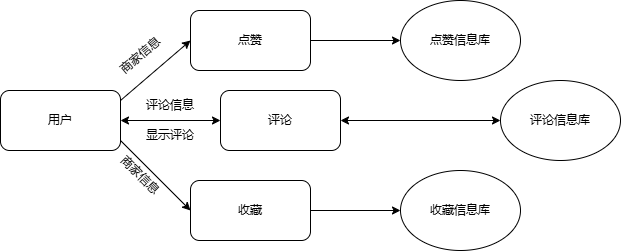
\includegraphics[width=5.76389in,height=2.32986in]{Picture38}

           图 9 点赞、评论和收藏功能细化数据流图

(8)商家功能

​  
功能描述:用户提交电话和密码触发商户登录事务,如果未进行注册则先进行注册事务,提交电话和密码至用户信息库。若进行过注册则进行比对,一致则登录成功。登陆事务出发后用户可以进行商户信息修改和上架商品等功能。

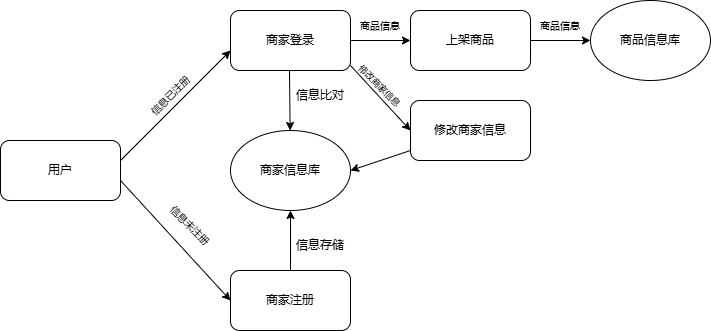
\includegraphics[width=5.76181in,height=2.68264in]{Picture39}

图 10 商家功能细化数据流图

\section{数据需求}

\subsection{静态数据}

用户信息、商户信息、点赞信息、收藏信息、评论信息、商品信息

\subsection{动态数据}

用户输入的搜索信息,输入框内的信息

\subsection{数据字典}

\section{数据流条目}

(1)身份信息

\begin{longtable}[]{@{}ll@{}}
\toprule
名称 & 身份信息\tabularnewline
简述 & 个人用户和商家用户的身份\tabularnewline
来源 & 个人用户和商家用户\tabularnewline
去处 & 用户登录\tabularnewline
\bottomrule
\end{longtable}

(2)用户名

\begin{longtable}[]{@{}ll@{}}
\toprule
名称 & 用户名\tabularnewline
简述 & 用户登录的账号\tabularnewline
类型 & varchar\tabularnewline
长度 & 1024\tabularnewline
来源 & 用户登录\tabularnewline
去处 & 用户信息库\tabularnewline
\bottomrule
\end{longtable}

(3)密码

\begin{longtable}[]{@{}ll@{}}
\toprule
名称 & 密码\tabularnewline
简述 & 用户登录的账号对应的密码\tabularnewline
类型 & varchar\tabularnewline
长度 & 1024\tabularnewline
来源 & 用户登录\tabularnewline
去处 & 用户信息库\tabularnewline
\bottomrule
\end{longtable}

(4)搜索商家

\begin{longtable}[]{@{}ll@{}}
\toprule
名称 & 搜索信息\tabularnewline
简述 & 用户发出搜索商户的信息\tabularnewline
来源 & 用户输入\tabularnewline
去处 & 搜索问题\tabularnewline
\bottomrule
\end{longtable}

(5)注册信息

\begin{longtable}[]{@{}ll@{}}
\toprule
名称 & 新用户注册信息\tabularnewline
简述 & 新用户进行注册的信息\tabularnewline
来源 & 用户输入\tabularnewline
去处 & 注册(用户信息库)\tabularnewline
\bottomrule
\end{longtable}

(6)点赞信息

\begin{longtable}[]{@{}ll@{}}
\toprule
名称 & 点赞信息\tabularnewline
简述 & 用户点赞时的信息\tabularnewline
来源 & 用户\tabularnewline
去处 & 点赞信息库\tabularnewline
\bottomrule
\end{longtable}

(7)收藏信息

\begin{longtable}[]{@{}ll@{}}
\toprule
名称 & 收藏信息\tabularnewline
简述 & 用户收藏时的信息\tabularnewline
来源 & 用户\tabularnewline
去处 & 收藏信息库\tabularnewline
\bottomrule
\end{longtable}

(8)评论信息

\begin{longtable}[]{@{}ll@{}}
\toprule
名称 & 评论信息\tabularnewline
简述 & 用户评论时的信息\tabularnewline
来源 & 用户输入\tabularnewline
去处 & 评论信息库\tabularnewline
\bottomrule
\end{longtable}

(9)商家列表

\begin{longtable}[]{@{}ll@{}}
\toprule
名称 & 商家列表\tabularnewline
简述 & 商家的信息列表\tabularnewline
来源 & 商家\tabularnewline
去处 & 查看商家\tabularnewline
\bottomrule
\end{longtable}

(10)商家信息

\begin{longtable}[]{@{}ll@{}}
\toprule
名称 & 商家信息\tabularnewline
简述 & 用户点单时展示的商家信息\tabularnewline
来源 & 商家\tabularnewline
去处 & 用户点单\tabularnewline
\bottomrule
\end{longtable}

(11)支付信息

\begin{longtable}[]{@{}ll@{}}
\toprule
名称 & 支付信息\tabularnewline
简述 & 进行支付时的信息\tabularnewline
来源 & 用户点单\tabularnewline
去处 & 用户支付\tabularnewline
\bottomrule
\end{longtable}

(12)订单信息

\begin{longtable}[]{@{}ll@{}}
\toprule
名称 & 订单信息\tabularnewline
简述 & 用户点单后产生的订单信息\tabularnewline
来源 & 用户点单\tabularnewline
去处 & 订单信息库\tabularnewline
\bottomrule
\end{longtable}

(13)AI咨询信息

\begin{longtable}[]{@{}ll@{}}
\toprule
名称 & AI咨询信息\tabularnewline
简述 & 用户输入的咨询问题\tabularnewline
来源 & 用户输入\tabularnewline
去处 & AI咨询\tabularnewline
\bottomrule
\end{longtable}

(14)个人信息

\begin{longtable}[]{@{}ll@{}}
\toprule
名称 & 个人信息\tabularnewline
简述 & 用户的个人信息展示\tabularnewline
来源 & 用户登录、用户信息库\tabularnewline
去处 & 我的信息功能\tabularnewline
\bottomrule
\end{longtable}

(15)修改的个人信息

\begin{longtable}[]{@{}ll@{}}
\toprule
名称 & 修改的个人信息\tabularnewline
简述 & 用户输入的新用户信息\tabularnewline
来源 & 我的信息中用户输入\tabularnewline
去处 & 我的信息功能\tabularnewline
\bottomrule
\end{longtable}

(16)商户用户名

\begin{longtable}[]{@{}ll@{}}
\toprule
名称 & 商户用户名\tabularnewline
简述 & 商户的电话号码\tabularnewline
来源 & 商户注册时的用户名\tabularnewline
去处 & 商户登录\tabularnewline
\bottomrule
\end{longtable}

(17)商户注册

\begin{longtable}[]{@{}ll@{}}
\toprule
名称 & 商户注册信息\tabularnewline
简述 & 商户注册时信息\tabularnewline
来源 & 商户输入\tabularnewline
去处 & 商户登录\tabularnewline
\bottomrule
\end{longtable}

(18)商户密码

\begin{longtable}[]{@{}ll@{}}
\toprule
名称 & 商户密码\tabularnewline
简述 & 商户登录的账号对应的密码\tabularnewline
类型 & varchar\tabularnewline
长度 & 1024\tabularnewline
来源 & 商户登录\tabularnewline
去处 & 商家信息库\tabularnewline
\bottomrule
\end{longtable}

(19)商品信息

\begin{longtable}[]{@{}ll@{}}
\toprule
名称 & 商品信息\tabularnewline
简述 & 商户商品的详细信息\tabularnewline
来源 & 商户\tabularnewline
去处 & 商品信息库\tabularnewline
\bottomrule
\end{longtable}

(20)上架商品信息

\begin{longtable}[]{@{}ll@{}}
\toprule
名称 & 上架商品信息\tabularnewline
简述 & 商户想要上架的商品信息\tabularnewline
来源 & 上架商品\tabularnewline
去处 & 商品信息库\tabularnewline
\bottomrule
\end{longtable}

(21)地址信息

\begin{longtable}[]{@{}ll@{}}
\toprule
名称 & 地址信息\tabularnewline
简述 & 外卖配送地址\tabularnewline
来源 & 地址添加\tabularnewline
去处 & 点餐功能\tabularnewline
\bottomrule
\end{longtable}

\section{数据存储条目}

(1)用户信息

\begin{longtable}[]{@{}ll@{}}
\toprule
名称 & 用户信息\tabularnewline
简述 & 描述用户的信息\tabularnewline
组成 & 用户名+密码+昵称+头像+Id\tabularnewline
组织方式 & 以Id为关键字\tabularnewline
\bottomrule
\end{longtable}

(2)地址信息

\begin{longtable}[]{@{}ll@{}}
\toprule
名称 & 地址信息\tabularnewline
简述 & 描述配送地址的信息\tabularnewline
组成 & 名称+电话+地址+编号\tabularnewline
组织方式 & 以编号为关键字\tabularnewline
\bottomrule
\end{longtable}

(3)商户信息

\begin{longtable}[]{@{}ll@{}}
\toprule
名称 & 用户信息\tabularnewline
简述 & 描述商家的信息\tabularnewline
组成 & 编号+图片+地址+类别+名称+商品+电话+密码\tabularnewline
组织方式 & 以编号为关键字\tabularnewline
\bottomrule
\end{longtable}

(4)商品信息

\begin{longtable}[]{@{}ll@{}}
\toprule
名称 & 商品信息\tabularnewline
简述 & 描述商品的信息\tabularnewline
组成 & 商品名称+编号+商户+图片\tabularnewline
组织方式 & 以编号为关键字\tabularnewline
\bottomrule
\end{longtable}

(5)点赞信息

\begin{longtable}[]{@{}ll@{}}
\toprule
名称 & 点赞信息\tabularnewline
简述 & 描述商家获得点赞的信息\tabularnewline
组成 & 用户编号+商家编号+点赞编号\tabularnewline
组织方式 & 以点赞编号为关键字\tabularnewline
\bottomrule
\end{longtable}

(6)收藏信息

\begin{longtable}[]{@{}ll@{}}
\toprule
名称 & 收藏信息\tabularnewline
简述 & 描述商家获得收藏的信息\tabularnewline
组成 & 用户编号+商家编号+收藏编号\tabularnewline
组织方式 & 以收藏编号为关键字\tabularnewline
\bottomrule
\end{longtable}

(7)评论信息

\begin{longtable}[]{@{}ll@{}}
\toprule
名称 & 评论信息\tabularnewline
简述 & 描述商家获得评论的信息\tabularnewline
组成 & 用户编号+商家编号+评论编号\tabularnewline
组织方式 & 以评论编号为关键字\tabularnewline
\bottomrule
\end{longtable}

\section{性能需求}

\subsection{数据精度}

\begin{longtable}[]{@{}lll@{}}
\toprule
字段 & 精度 & 备注\tabularnewline
用户名 & char型 & 符合中国大陆电话格式\tabularnewline
密码 & char型 & 8位以上,大小写、符号和数字都要包含\tabularnewline
昵称 & char型 & 8位以下\tabularnewline
用户是否存在 & map型 &
前端传过来含有用户名和密码的json对象,后端接受到之后在数据库中匹配,返回是否匹配的信息给前端\tabularnewline
用户ID & int型 & 自动赋值\tabularnewline
\bottomrule
\end{longtable}

\subsection{时间特性}

(1) 响应时间:用户任意操作后2秒内系统给予反馈信息。

(2) 更新处理时间:由系统运行状态来决定。

(3) 数据的转换和传送时间:能够在5秒内完成。

5.3 灵活性

  
当需求发生某些变化时,该软件的基本操作、数据结构、运行环境等等基本不会发生变化,只是对系统的数据库的文件和记录进行处理,就可以满足需求。

\section{运行需求}

\subsection{用户界面}


\begin{quote}
(1)注册:用户填写该页面的``用户名''、``昵称''、``密码''、``确认密码''、``头像''信息后点击提交即可成功注册,返回``注册是否成功的消息''。

(2)登录:用户填写该页面的``用户名''、``密码''信息后点击登录即可成功登录,如果用户没有账号可以点击下方按钮进行注册。

(3)主页:该页面展示各个不同种类的美食,底部显示主页、发现、订单、我的四个按钮,右上角显示登录注册按钮,可以进入不同的页面。

(4)个人中心:点击修改资料可以修改资料;中间提供展示该用户的基本数据信息;点击最下方的退出可以登出用户。

(5)点单流程:点击后展示每个类别的商家列表,再进一步点击可以展示商家的商品信息,并可以进行点单,进入支付页面并完成支付。

(6)AI咨询:点击首页发现键进入AI界面,可以输入想要咨询的问题并发送,返回的内容会被显示在下方。

(7)我的订单:订单界面分别显示已支付订单和未支付订单,并且可以点击下拉按钮显示订单明细,对于未支付订单可以点击去支付完成订单的支付。

(8)商户信息:进行商户登陆后会显示该商户的基本信息,如图片、名称以及电话和菜品等。

(9)上架商品:商家登陆后可以上架新商品,输入新商品的图片、价格、名称和简介即可上架。
\end{quote}

(10)搜索商户:用户可以在首页的搜索栏输入搜索内容,点击搜索后下方展示搜索出的商家,并可以点击商家进行点餐。

\subsection{软件接口}

1.操作系统:Microsoft Windows系统

2.软件设备:VScode、IntelliJ IDEA、MySQL8.0、eclipse

\subsection{质量属性}

1.可用性:用户可以使用

2.可靠性:在给定时间内可以满足无错运行的要求

3.可维护性:服务器重启、写进日志

4.安全性:对用户的密码加密

5.可移植性:移动端移植



